\documentclass[10pt]{article}
\usepackage[usenames]{color} %used for font color
\usepackage{amssymb} %maths
\usepackage{amsmath} %maths
\usepackage[utf8]{inputenc} %useful to type directly diacritic characters
\usepackage{tikz}
\usetikzlibrary{arrows,positioning,decorations.pathreplacing} 

\definecolor{boiseBlue} {RGB}{29,72,159}
\definecolor{rojoAmor} {RGB}{171,13,4}
\definecolor{moradoAmor} {RGB}{93,8,113}
\definecolor{verdeAmor} {RGB}{98,158,31}
\definecolor{negro} {RGB}{10,10,10}
\definecolor{lgreen} {RGB}{180,210,100}
\definecolor{dblue}  {RGB}{20,66,129}
\definecolor{ddblue} {RGB}{11,36,69}
\definecolor{lred}   {RGB}{220,0,0}
\definecolor{nred}   {RGB}{224,0,0}
\definecolor{norange}{RGB}{230,120,20}
\definecolor{nyellow}{RGB}{255,221,0}
\definecolor{ngreen} {RGB}{98,158,31}
\definecolor{dgreen} {RGB}{78,138,21}
\definecolor{nblue}  {RGB}{28,130,185}
\definecolor{jblue}  {RGB}{20,50,100}\begin{document}
\[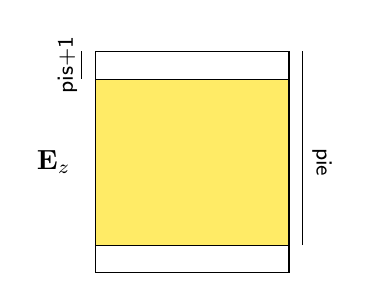
\begin{tikzpicture}
%
\node[draw=black,minimum width=7em,minimum height=8em,rectangle]  at (0,0) {};
\node[draw=black,fill=nyellow!60,minimum width=7em,minimum height=6em,rectangle]  at (0,0) {};
%
\node[]  at (-5em,0) {${\bf E}_z$};
%
\draw[] (-4em,4em) -- (-4em,3em);
%\draw[] (-3.5em,4.5em) -- (-2.5em,4.5em);
%\draw[] (-2.5em,-4.5em) -- (3.5em,-4.5em);
\draw[] (4em,-3em) -- (4em,4em);
%
%\node[]  at (0.5em,-5.5em) {\footnotesize{{\sf ny}}};
\node[rotate=-90]  at (4.7em,0) {\footnotesize{{\sf pie}}};
\node[rotate=90]  at (-4.5em,3.5em) {\footnotesize{{\sf pis+1}}};
%\node[]  at (-3em,5em) {\footnotesize{1}};
\end{tikzpicture}
\]
\end{document}